\documentclass{standalone}
\usepackage{tikz}
\usetikzlibrary{patterns, positioning}

\begin{document}
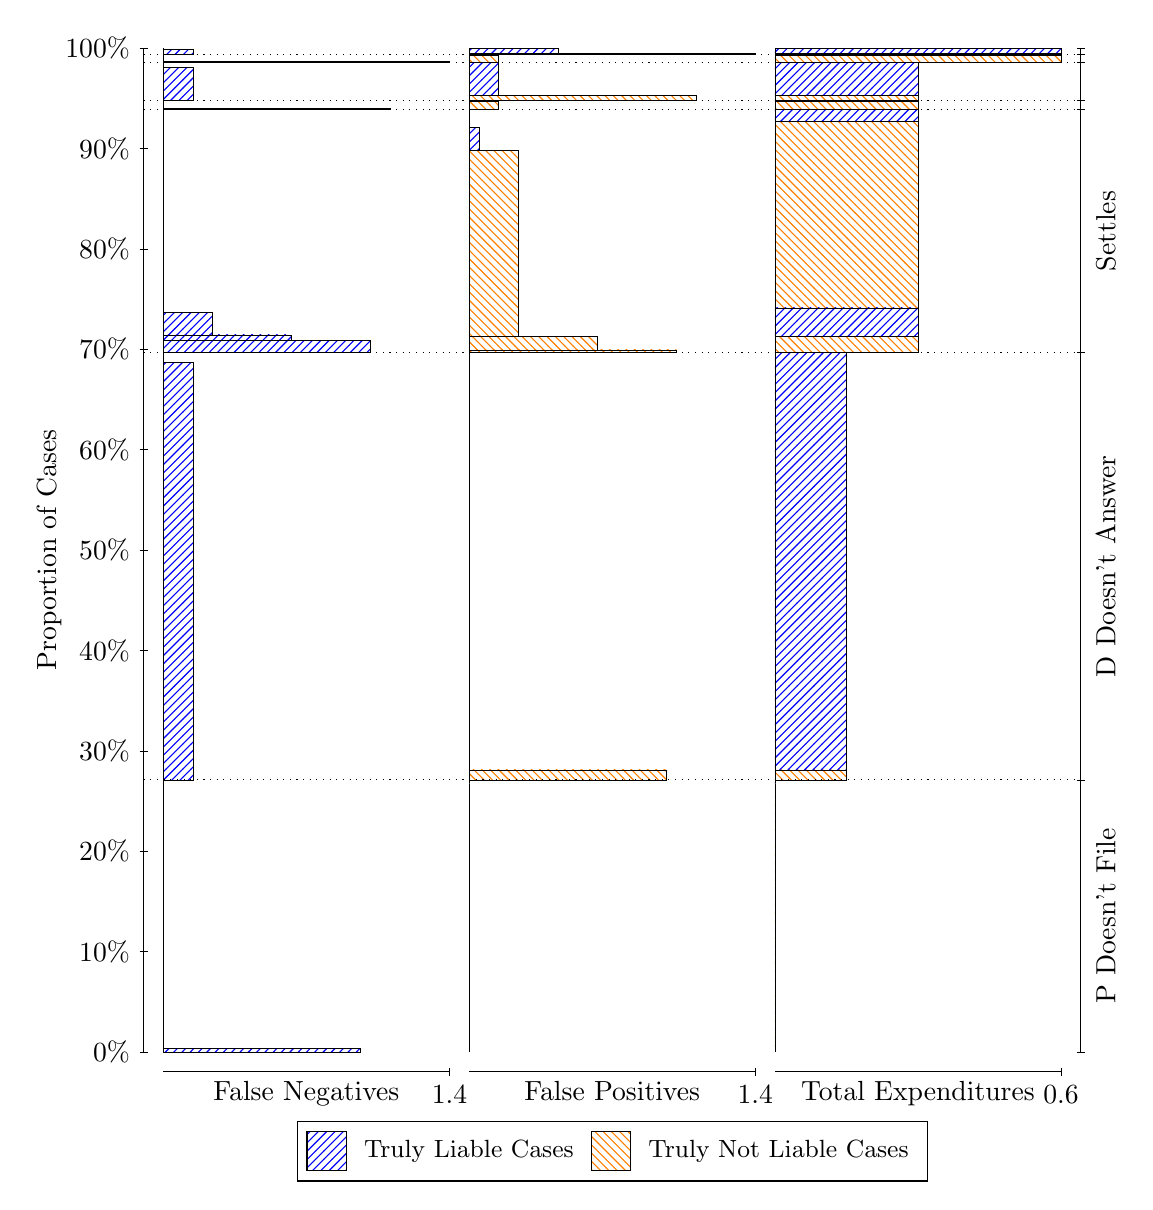
\begin{tikzpicture}
\draw[black, very thin] (1.5,1.75) -- (1.5,14.5);
\node[rotate=90, anchor=center] at (0.3, 8.125) {Proportion of Cases};
\draw[black, very thin] (1.45,1.75) -- (1.55,1.75);
\node[anchor=east] at (1.45, 1.75) {0\%};
\draw[black, very thin] (1.45,3.025) -- (1.55,3.025);
\node[anchor=east] at (1.45, 3.025) {10\%};
\draw[black, very thin] (1.45,4.3) -- (1.55,4.3);
\node[anchor=east] at (1.45, 4.3) {20\%};
\draw[black, very thin] (1.45,5.575) -- (1.55,5.575);
\node[anchor=east] at (1.45, 5.575) {30\%};
\draw[black, very thin] (1.45,6.85) -- (1.55,6.85);
\node[anchor=east] at (1.45, 6.85) {40\%};
\draw[black, very thin] (1.45,8.125) -- (1.55,8.125);
\node[anchor=east] at (1.45, 8.125) {50\%};
\draw[black, very thin] (1.45,9.4) -- (1.55,9.4);
\node[anchor=east] at (1.45, 9.4) {60\%};
\draw[black, very thin] (1.45,10.675) -- (1.55,10.675);
\node[anchor=east] at (1.45, 10.675) {70\%};
\draw[black, very thin] (1.45,11.95) -- (1.55,11.95);
\node[anchor=east] at (1.45, 11.95) {80\%};
\draw[black, very thin] (1.45,13.225) -- (1.55,13.225);
\node[anchor=east] at (1.45, 13.225) {90\%};
\draw[black, very thin] (1.45,14.5) -- (1.55,14.5);
\node[anchor=east] at (1.45, 14.5) {100\%};

\draw[black, very thin] (13.4,1.75) -- (13.4,14.5);
\draw[black, very thin] (13.35,1.75) -- (13.45,1.75);
\node[anchor=west] at (13.35, 1.75) {};
\draw[black, very thin] (13.35,5.2061) -- (13.45,5.2061);
\node[anchor=west] at (13.35, 5.2061) {};
\draw[black, very thin] (13.35,10.634) -- (13.45,10.634);
\node[anchor=west] at (13.35, 10.634) {};
\draw[black, very thin] (13.35,13.717) -- (13.45,13.717);
\node[anchor=west] at (13.35, 13.717) {};
\draw[black, very thin] (13.35,13.836) -- (13.45,13.836);
\node[anchor=west] at (13.35, 13.836) {};
\draw[black, very thin] (13.35,14.319) -- (13.45,14.319);
\node[anchor=west] at (13.35, 14.319) {};
\draw[black, very thin] (13.35,14.416) -- (13.45,14.416);
\node[anchor=west] at (13.35, 14.416) {};
\draw[black, very thin] (13.35,14.5) -- (13.45,14.5);
\node[anchor=west] at (13.35, 14.5) {};

\draw[black, very thin, pattern color=blue, pattern=north east lines] (1.75,1.75) rectangle (4.2557,1.7989);
\draw[black, very thin, pattern color=orange, pattern=north west lines] (1.75,1.7989) rectangle (1.75,5.2061);
\draw[black, very thin, pattern color=blue, pattern=north east lines] (1.75,5.2061) rectangle (2.1259,10.507);
\draw[black, very thin, pattern color=orange, pattern=north west lines] (1.75,10.507) rectangle (1.75,10.634);
\draw[black, very thin, pattern color=blue, pattern=north east lines] (1.75,10.634) rectangle (4.381,10.784);
\draw[black, very thin, pattern color=blue, pattern=north east lines] (1.75,10.784) rectangle (3.3787,10.856);
\draw[black, very thin, pattern color=blue, pattern=north east lines] (1.75,10.856) rectangle (2.3764,11.147);
\draw[black, very thin, pattern color=orange, pattern=north west lines] (1.75,11.147) rectangle (1.75,13.717);
\draw[black, very thin, pattern color=blue, pattern=north east lines] (1.75,13.717) rectangle (4.6316,13.731);
\draw[black, very thin, pattern color=orange, pattern=north west lines] (1.75,13.731) rectangle (1.75,13.836);
\draw[black, very thin, pattern color=blue, pattern=north east lines] (1.75,13.836) rectangle (2.1259,14.252);
\draw[black, very thin, pattern color=orange, pattern=north west lines] (1.75,14.252) rectangle (1.75,14.319);
\draw[black, very thin, pattern color=blue, pattern=north east lines] (1.75,14.319) rectangle (5.3833,14.333);
\draw[black, very thin, pattern color=orange, pattern=north west lines] (1.75,14.333) rectangle (1.75,14.416);
\draw[black, very thin, pattern color=blue, pattern=north east lines] (1.75,14.416) rectangle (2.1259,14.485);
\draw[black, very thin, pattern color=orange, pattern=north west lines] (1.75,14.485) rectangle (1.75,14.5);
\draw[black, very thin, pattern color=orange, pattern=north west lines] (5.6333,1.75) rectangle (5.6333,5.1571);
\draw[black, very thin, pattern color=blue, pattern=north east lines] (5.6333,5.1571) rectangle (5.6333,5.2061);
\draw[black, very thin, pattern color=orange, pattern=north west lines] (5.6333,5.2061) rectangle (8.1391,5.3339);
\draw[black, very thin, pattern color=blue, pattern=north east lines] (5.6333,5.3339) rectangle (5.6333,10.634);
\draw[black, very thin, pattern color=orange, pattern=north west lines] (5.6333,10.634) rectangle (8.2644,10.666);
\draw[black, very thin, pattern color=orange, pattern=north west lines] (5.6333,10.666) rectangle (7.2621,10.837);
\draw[black, very thin, pattern color=orange, pattern=north west lines] (5.6333,10.837) rectangle (6.2598,13.204);
\draw[black, very thin, pattern color=blue, pattern=north east lines] (5.6333,13.204) rectangle (5.7586,13.496);
\draw[black, very thin, pattern color=blue, pattern=north east lines] (5.6333,13.496) rectangle (5.6333,13.717);
\draw[black, very thin, pattern color=orange, pattern=north west lines] (5.6333,13.717) rectangle (6.0092,13.822);
\draw[black, very thin, pattern color=blue, pattern=north east lines] (5.6333,13.822) rectangle (5.6333,13.836);
\draw[black, very thin, pattern color=orange, pattern=north west lines] (5.6333,13.836) rectangle (8.5149,13.903);
\draw[black, very thin, pattern color=blue, pattern=north east lines] (5.6333,13.903) rectangle (6.0092,14.319);
\draw[black, very thin, pattern color=orange, pattern=north west lines] (5.6333,14.319) rectangle (6.0092,14.402);
\draw[black, very thin, pattern color=blue, pattern=north east lines] (5.6333,14.402) rectangle (5.6333,14.416);
\draw[black, very thin, pattern color=orange, pattern=north west lines] (5.6333,14.416) rectangle (9.2667,14.431);
\draw[black, very thin, pattern color=blue, pattern=north east lines] (5.6333,14.431) rectangle (6.7609,14.5);
\draw[black, very thin, pattern color=orange, pattern=north west lines] (9.5167,1.75) rectangle (9.5167,5.1571);
\draw[black, very thin, pattern color=blue, pattern=north east lines] (9.5167,5.1571) rectangle (9.5167,5.2061);
\draw[black, very thin, pattern color=orange, pattern=north west lines] (9.5167,5.2061) rectangle (10.425,5.3339);
\draw[black, very thin, pattern color=blue, pattern=north east lines] (9.5167,5.3339) rectangle (10.425,10.634);
\draw[black, very thin, pattern color=orange, pattern=north west lines] (9.5167,10.634) rectangle (11.333,10.837);
\draw[black, very thin, pattern color=blue, pattern=north east lines] (9.5167,10.837) rectangle (11.333,11.2);
\draw[black, very thin, pattern color=orange, pattern=north west lines] (9.5167,11.2) rectangle (11.333,13.567);
\draw[black, very thin, pattern color=blue, pattern=north east lines] (9.5167,13.567) rectangle (11.333,13.717);
\draw[black, very thin, pattern color=orange, pattern=north west lines] (9.5167,13.717) rectangle (11.333,13.822);
\draw[black, very thin, pattern color=blue, pattern=north east lines] (9.5167,13.822) rectangle (11.333,13.836);
\draw[black, very thin, pattern color=orange, pattern=north west lines] (9.5167,13.836) rectangle (11.333,13.903);
\draw[black, very thin, pattern color=blue, pattern=north east lines] (9.5167,13.903) rectangle (11.333,14.319);
\draw[black, very thin, pattern color=orange, pattern=north west lines] (9.5167,14.319) rectangle (13.15,14.402);
\draw[black, very thin, pattern color=blue, pattern=north east lines] (9.5167,14.402) rectangle (13.15,14.416);
\draw[black, very thin, pattern color=orange, pattern=north west lines] (9.5167,14.416) rectangle (13.15,14.431);
\draw[black, very thin, pattern color=blue, pattern=north east lines] (9.5167,14.431) rectangle (13.15,14.5);
\draw[black, dotted] (1.5,5.2061) -- (13.4,5.2061);
\draw[black, dotted] (1.5,10.634) -- (13.4,10.634);
\draw[black, dotted] (1.5,13.717) -- (13.4,13.717);
\draw[black, dotted] (1.5,13.836) -- (13.4,13.836);
\draw[black, dotted] (1.5,14.319) -- (13.4,14.319);
\draw[black, dotted] (1.5,14.416) -- (13.4,14.416);
\draw[black, very thin] (1.75,1.5) -- (5.3833,1.5);
\node[anchor=north] at (3.5667, 1.5) {False Negatives};
\draw[black, very thin] (5.3833,1.45) -- (5.3833,1.55);
\node[anchor=north] at (5.3833, 1.45) {1.4};

\draw[black, very thin] (5.6333,1.5) -- (9.2667,1.5);
\node[anchor=north] at (7.45, 1.5) {False Positives};
\draw[black, very thin] (9.2667,1.45) -- (9.2667,1.55);
\node[anchor=north] at (9.2667, 1.45) {1.4};

\draw[black, very thin] (9.5167,1.5) -- (13.15,1.5);
\node[anchor=north] at (11.333, 1.5) {Total Expenditures};
\draw[black, very thin] (13.15,1.45) -- (13.15,1.55);
\node[anchor=north] at (13.15, 1.45) {0.6};

\node[black, centered, rotate=90] at (13.72, 3.478) {P Doesn't File};
\node[black, centered, rotate=90] at (13.72, 7.9202) {D Doesn't Answer};
\node[black, centered, rotate=90] at (13.72, 12.176) {Settles};





\draw (7.449999999999999,1.5) node[draw=none] (baseCoordinate) {};
\begin{scope}[align=center]
        \matrix[scale=0.5, draw=black, below=0.5cm of baseCoordinate, nodes={draw}, column sep=0.1cm]{
            \node[rectangle, draw, minimum width=0.5cm, minimum height=0.5cm, pattern=north east lines, pattern color=blue] {}; &
            \node[draw=none, font=\small] (B) {Truly Liable Cases}; &
            \node[rectangle, draw, minimum width=0.5cm, minimum height=0.5cm, pattern=north west lines, pattern color=orange] {}; &
            \node[draw=none, font=\small] (B) {Truly Not Liable Cases}; \\
            };
\end{scope}

\end{tikzpicture}
\end{document}